\section{Neural Networks}
\textbf{Date:} \underline{Oct 2, 2025}

\subsection{Multi-Layer Neural Networks}

\begin{center}
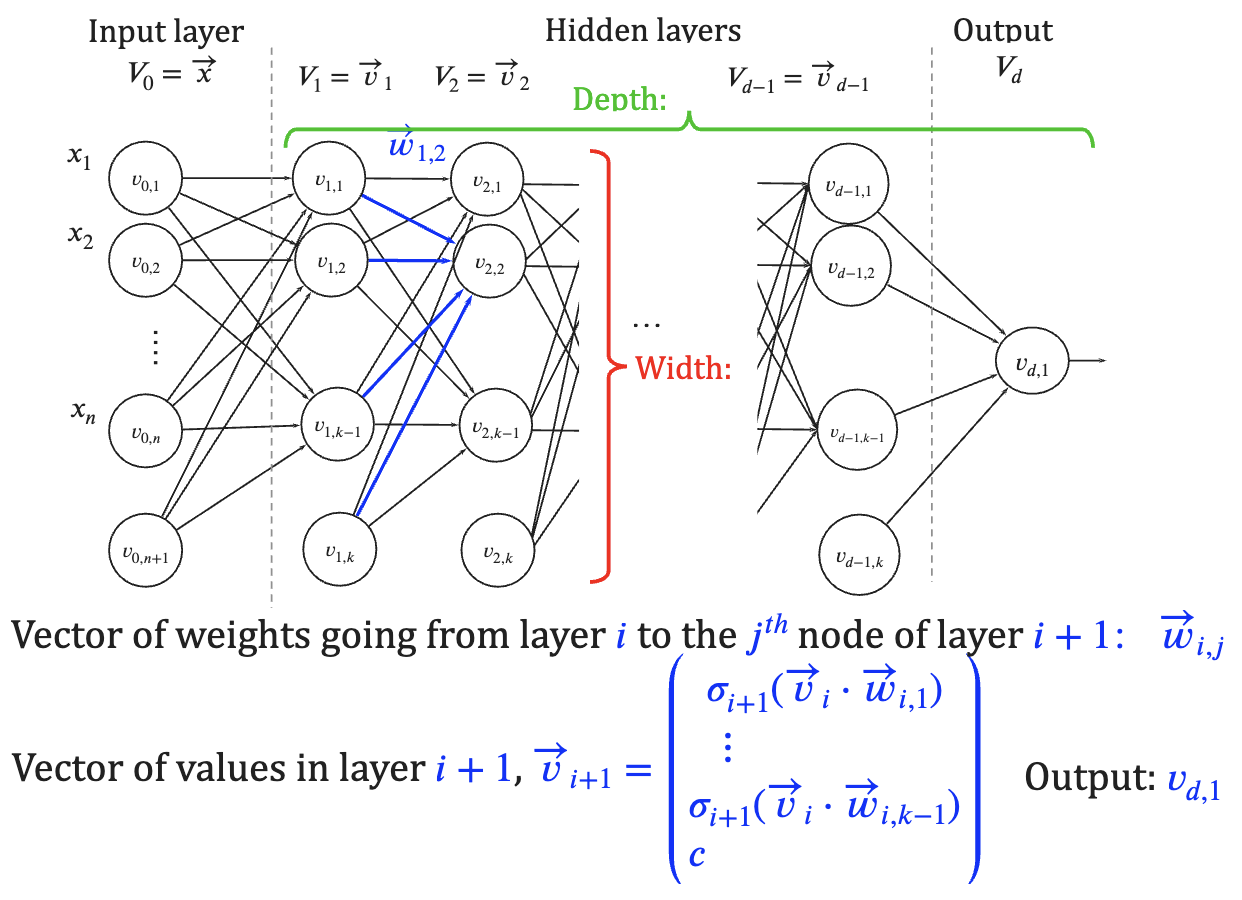
\includegraphics[width=0.6\textwidth]{Images/nn.png}
\end{center}

A multi-layer neural network (also called a feedforward neural network) consists of an input layer, one or more hidden layers, and an output layer. Each layer is made up of nodes (neurons), and each node in a layer is connected to every node in the next layer.
\begin{itemize}
    \item Let $\vec{v}_i$ be the vector of values in layer $i$.
    \item Let $\vec{w}_{i,j}$ be the vector of weights from layer $i$ to the $j$th node of layer $i+1$.
    \item The value at node $j$ in layer $i+1$ is computed as:
    \[
    v_{i+1, j} = \sigma_{i+1}(\vec{v}_i \cdot \vec{w}_{i,j})
    \]
    where $\sigma_{i+1}$ is the activation function for layer $i+1$.
\end{itemize}

\paragraph{Concise Matrix Formulation}

\begin{itemize}
    \item Let $W_i$ be the weight matrix for layer $i$, where each column $j$ is the weight vector $\vec{w}_{i,j}$.
    \item Layers are fully connected; any missing edge has weight $0$.
    \item The vector of activations for layer $i+1$ is:
    \[
    \vec{v}_{i+1} = \sigma_{i+1}(W_i^\top \vec{v}_i)
    \]
    where $\sigma_{i+1}$ is applied elementwise.
\end{itemize}


The output of a $d$-layer neural network can be written as a nested composition of linear transformations and activation functions:
\[
\sigma_d\left(W_{d-1}^\top \cdots\, \sigma_3\left(W_2^\top\, \sigma_2\left(W_1^\top\, \sigma_1\left(W_0^\top\, \vec{v}_0\right)\right)\right)\cdots\right)
\]
where each $\sigma_i$ is applied elementwise, and $W_i$ is the weight matrix for layer $i$.

\begin{algobox}
\textbf{Forward Propagation Algorithm:}

\textbf{Input:} Neural Network with weight matrices $W_0, W_1, \ldots, W_{d-1}$, activation functions $\sigma_1, \ldots, \sigma_d$ and instance $\vec{x}$

$\vec{v}_0 = \vec{x}$

\textbf{For} $\ell = 1, \ldots, d$
\begin{itemize}
    \item $\vec{s}_\ell = W_{\ell-1}^\top \vec{v}_{\ell-1}$
    \item $\vec{v}_\ell = \sigma_\ell(\vec{s}_\ell)$
\end{itemize}
\textbf{End For}

\textbf{Output} $\vec{v}_d$
\end{algobox}

\subsection{Non-linear Activation Functions}

Activation functions are applied to the nodes of a hidden layer in a neural network. They introduce non-linearity, allowing the network to learn complex patterns.

\begin{center}
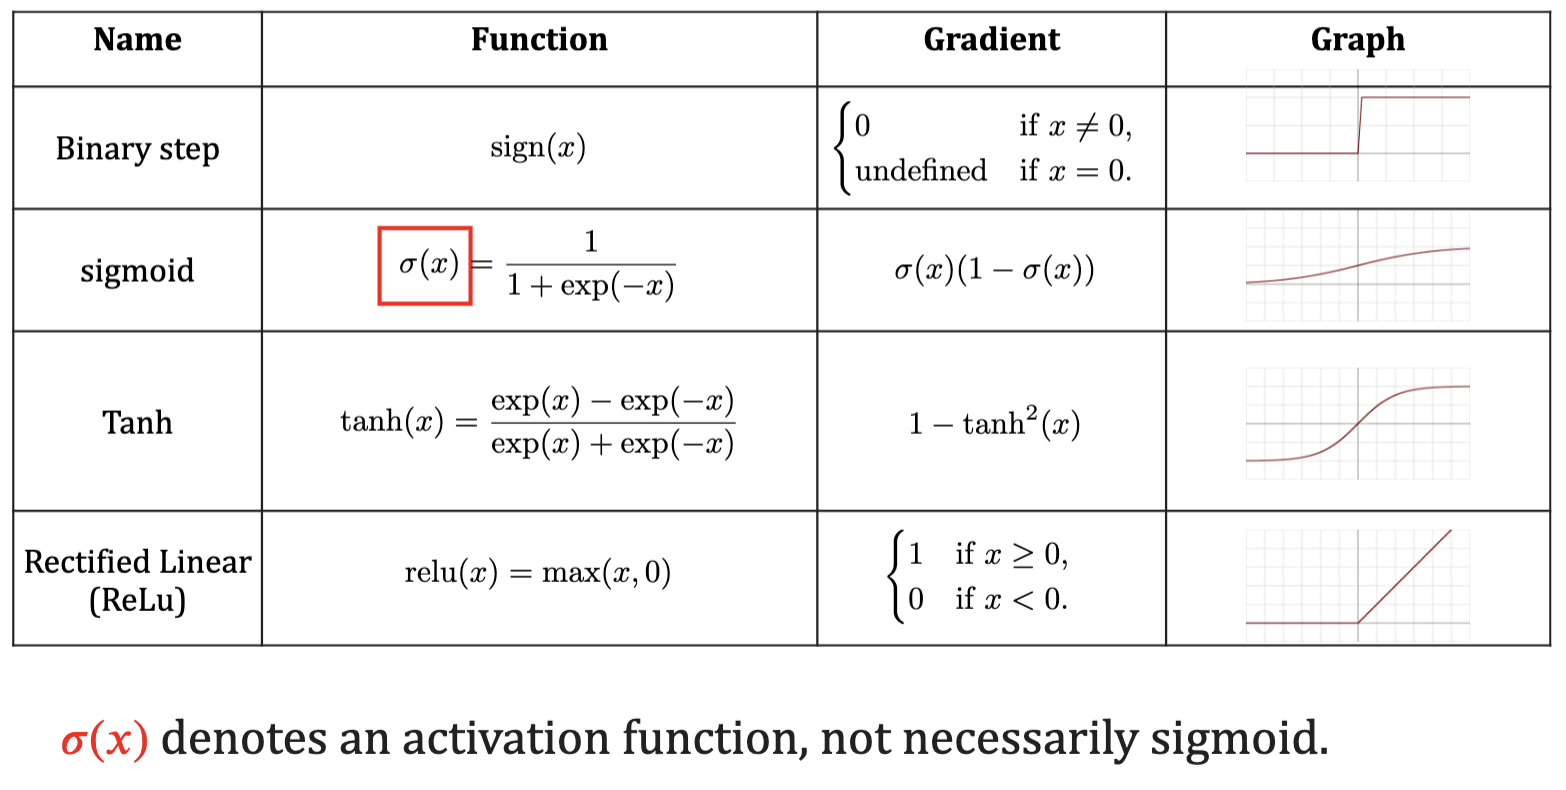
\includegraphics[width=0.6\textwidth]{Images/activations.png}
\end{center}

\begin{itemize}
    \item \textbf{Binary step:} Outputs 0 or 1, not differentiable at $x=0$.
    \item \textbf{Sigmoid:} Smooth, outputs between 0 and 1, can cause vanishing gradients.
    \item \textbf{Tanh:} Outputs between -1 and 1, zero-centered.
    \item \textbf{ReLU:} Simple, efficient, helps with vanishing gradient, but can "die" for negative inputs.
\end{itemize}

Deeper neural networks can express more complex functions only if we use non-linear activation.

If all activation functions are linear, then a multi-layer neural network is equivalent to a single-layer linear model. This is because a linear function of linear functions is still linear.

\textbf{Example:} Suppose the activation in the hidden layer is linear, $\sigma_1(x) = x$, and the output activation is non-linear, e.g., $\sigma_2(x) = \mathrm{sign}(x)$. Then, the output can be written as:
\[
v_{\text{out}} = \mathrm{sign}(\bar{w}_1 v_1 + \bar{w}_2 v_2) = \mathrm{sign}\left(\bar{w}_1(\vec{x} \cdot \vec{w} + b) + \bar{w}_2(\vec{x} \cdot \vec{w}' + b')\right)
\]
\[
= \mathrm{sign}(\vec{z} \cdot \vec{x} + \beta)
\]
where $\vec{z} = \bar{w}_1 \vec{w} + \bar{w}_2 \vec{w}'$ and $\beta = \bar{w}_1 b + \bar{w}_2 b'$.



\subsection{Universal Approximators}

A fundamental result in neural networks is the \textbf{Universal Approximation Theorem}. It states that a feedforward neural network with a single hidden layer (i.e., a depth-2 network) and a sufficiently large number of neurons (width) can approximate any continuous function on $\mathbb{R}^n$ to arbitrary accuracy, given appropriate activation functions (such as sigmoid or ReLU).

\textbf{How large does the hidden layer need to be?}
\begin{itemize}
    \item For boolean functions, the required width can be as large as $\exp(n)$, where $n$ is the input dimension.
    \item If we restrict ourselves to networks of polynomial size (i.e., width and number of parameters grow polynomially with $n$), then:
    \begin{itemize}
        \item We cannot approximate all possible functions.
        \item However, this restriction helps reduce the risk of overfitting.
        \item This tradeoff is known as the \textbf{bias-variance tradeoff}: larger networks can fit more complex functions (low bias, high variance), while smaller networks may generalize better (high bias, low variance).
    \end{itemize}
    \item Instead of fully connected layers, we can use structured networks (e.g., convolutional neural networks) to reduce the number of parameters and exploit structure in the data.
\end{itemize}
